\documentclass{article}
\usepackage[colorlinks=true,urlcolor=blue]{hyperref}
\usepackage[utf8]{inputenc}
\usepackage{subfig}
%References
\usepackage{natbib}
%IMPORTANT use https://www.citationmachine.net/ if you need to generate references!
% \citep{reference} creates Harvard Style references throughout

%Colors
\usepackage{xcolor}

\usepackage[protrusion=true,expansion]{microtype}

%Code Markup
\usepackage[outputdir=cache]{minted}
%Syntax Highlighting Style
\definecolor{bggray}{RGB}{40,40,40}
%Macro to make a Syntax Highlighter For Java files 
%Use \javacode{filename.java} to insert a Java File W/ Syntax Highlighting file into the PDF
\newmintedfile[javacode]{java}{
	style=fruity,
	bgcolor=bggray,
	linenos,
	breaklines,
	tabsize=2,
	obeytabs
}

\newmintedfile[cscode]{csharp}{
	style=fruity,
	bgcolor=bggray,
	linenos,
	breaklines,
	tabsize=2,
	obeytabs
}

\newmintedfile[bashoutput]{txt}{
	style=fruity,
	bgcolor=lightgray,
	breaklines,
	tabsize=2,
	obeytabs
}

%Page Margins and stuff
\usepackage{geometry}
 \geometry{
 a4paper,
 total={170mm,257mm},
 left=20mm,
 }

%Pictures
\usepackage{graphicx}
\graphicspath{ {./images/} }

%Move the title position
\usepackage{titling}

\setlength{\droptitle}{-8.5em} %Up, near the top but not too high

\title{CT3536 Games Programming - Game Dev Project}
\author{Daniel Hannon (19484286)}
\date{January 2022}

\begin{document}
	\maketitle
	\section{Overview}
	The game I wanted to make was Risk. The reason I wanted to do this was that I do not like the Steam Version of the game, linked \href{https://store.steampowered.com/app/1128810/RISK_Global_Domination/}{here}. A goal I made for myself was to make all of the assets (apart from the music, that was taken from Elder Scrolls IV Oblivion) \href{https://www.amazon.co.uk/dp/B07CT8Y3S4/ref=dm_ws_tlw_trk7}{here is a link to it}. Overall I got most of what I wanted to done and this will be discussed more in the reflection.
	\section{Creating the Assets}
	As I am not too experienced with creating assets, this was particularly challenging, I made the conscious decision to make the entire game 2D as I figured it would be easier to make 2D assets than 3D ones and it would contribute greatly to the aesthetic of the game. 
	\subsection{Making The Map}
	\begin{figure}[h!]
		\centering
		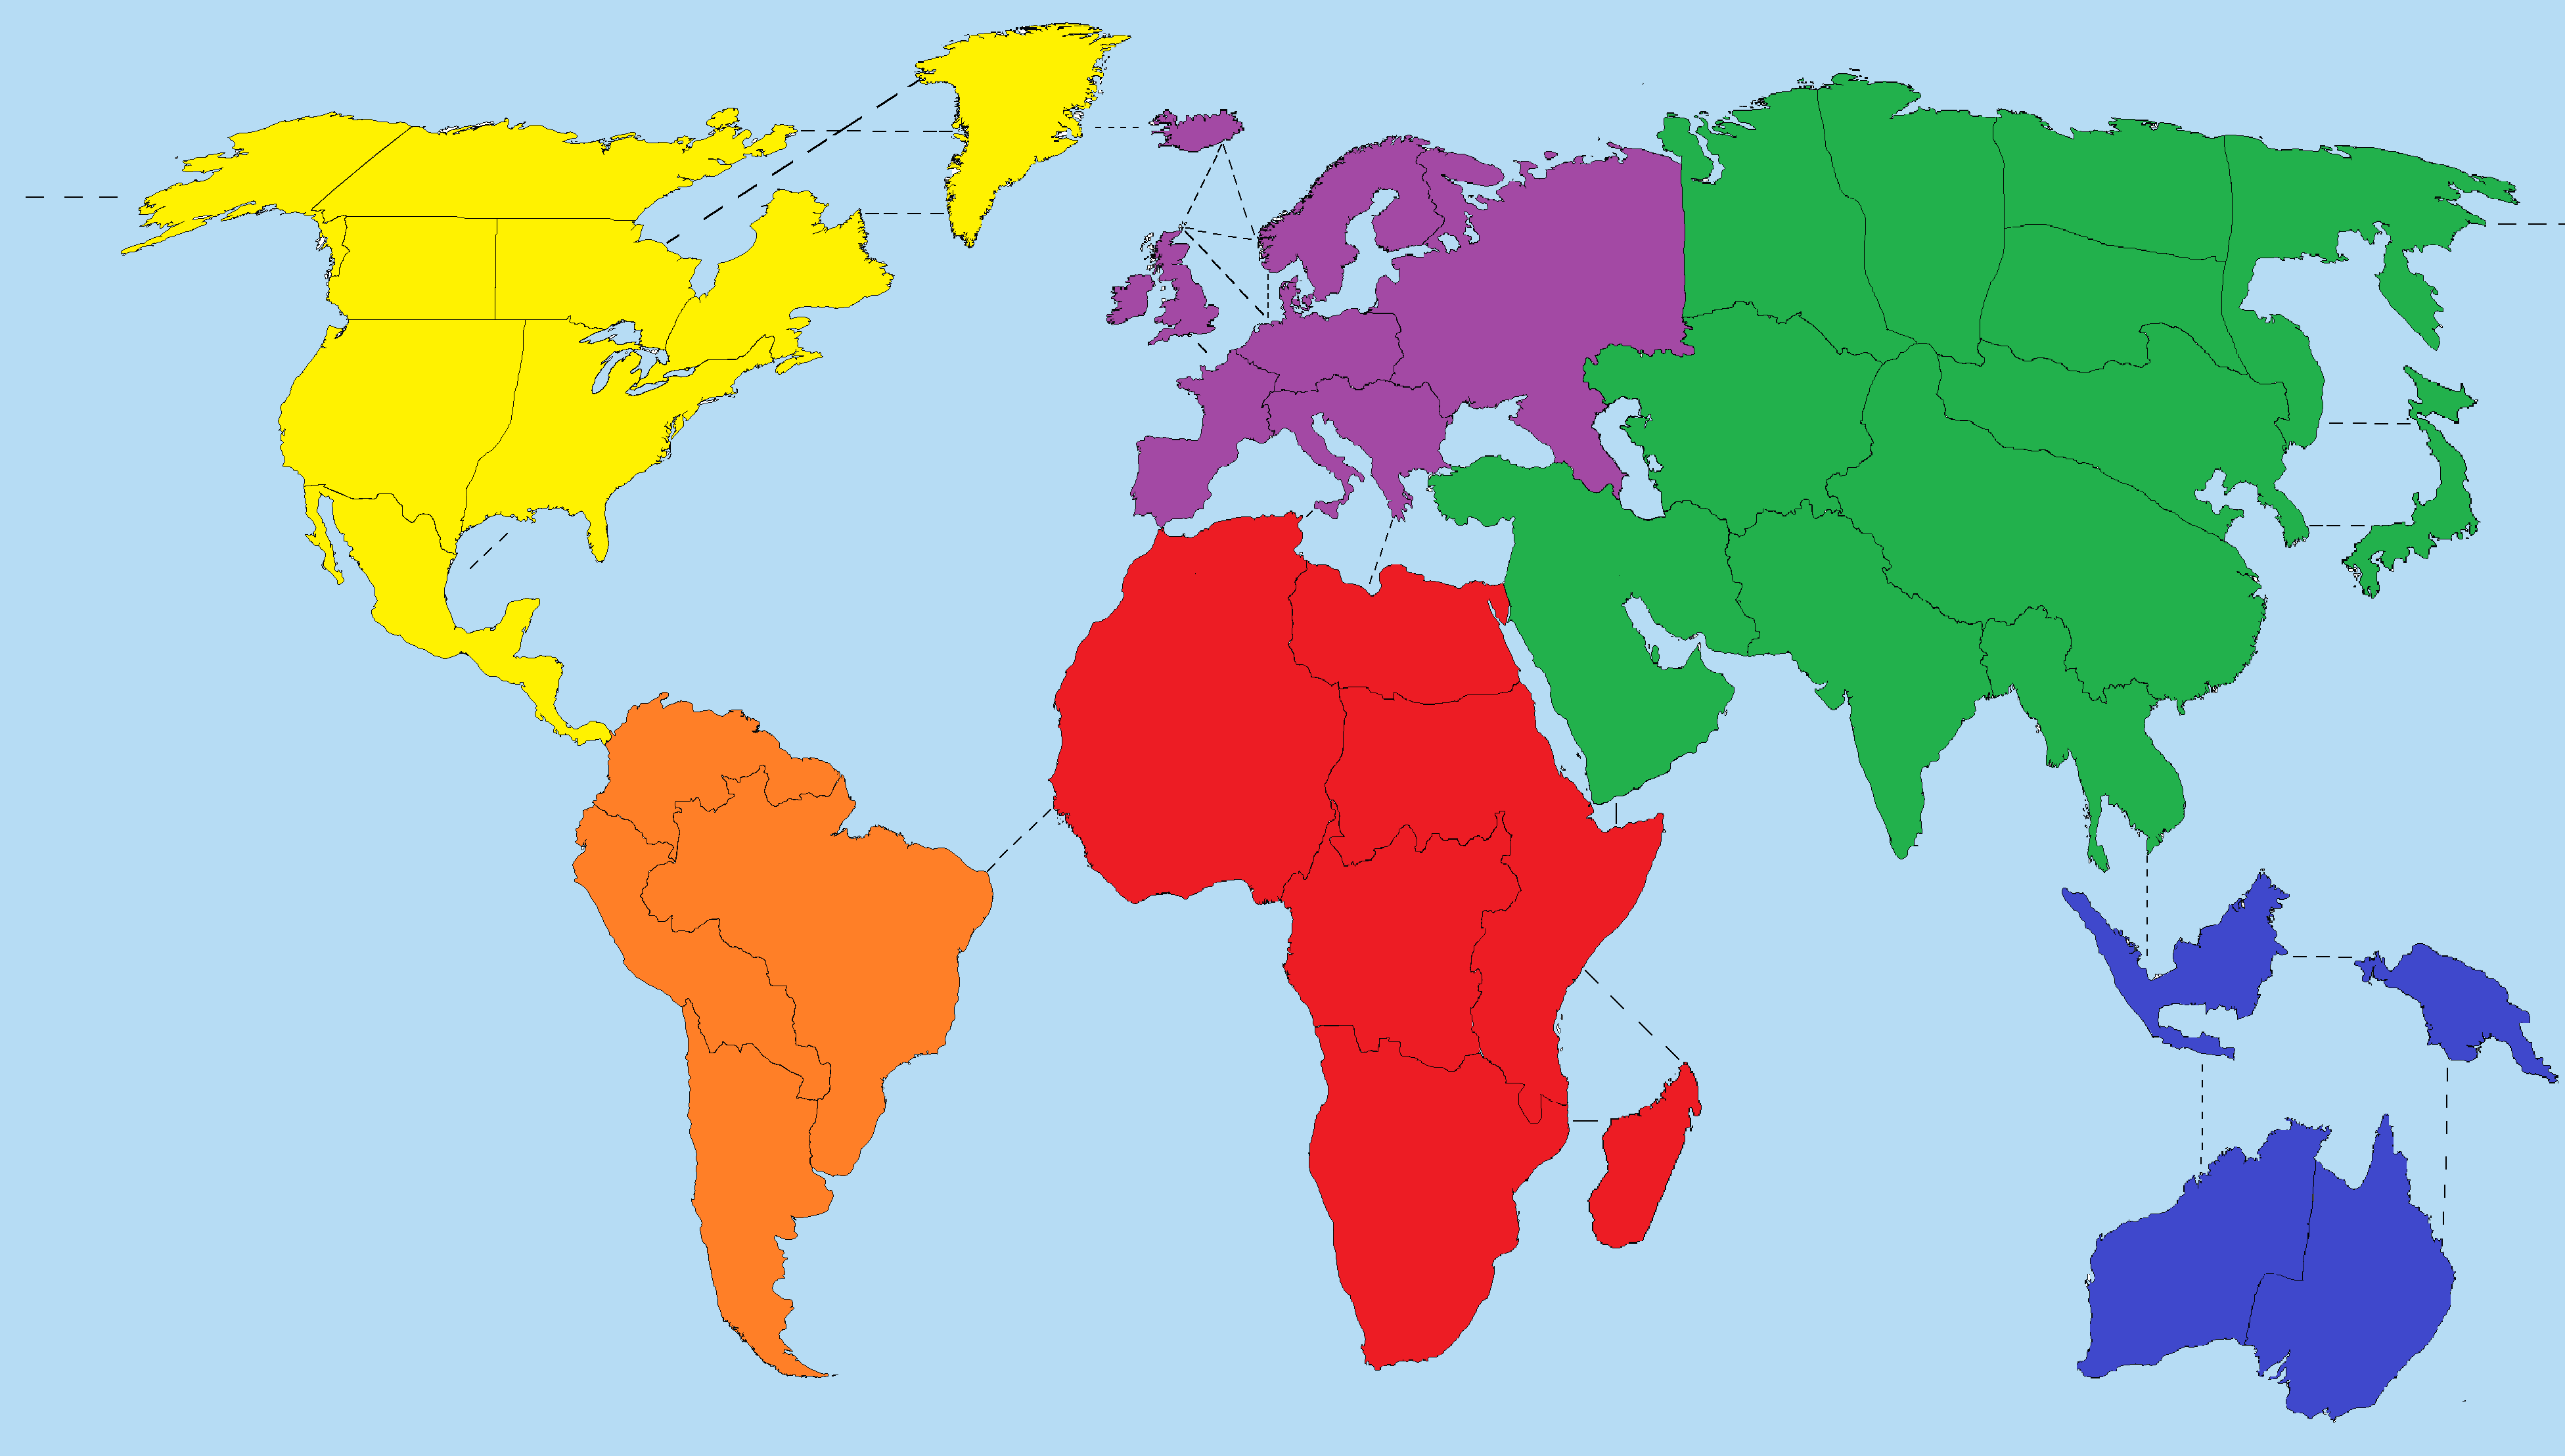
\includegraphics[width=0.7\textwidth]{final1.png}
	\end{figure}
	In Order to make a map that was as close to the risk board map as possible I needed something to work as a template, so I obtained a map from wikipedia (\href{https://upload.wikimedia.org/wikipedia/commons/c/cf/A_large_blank_world_map_with_oceans_marked_in_blue.PNG}{Source}) that looked like this:\\
	\begin{figure}[h!]
		\centering
		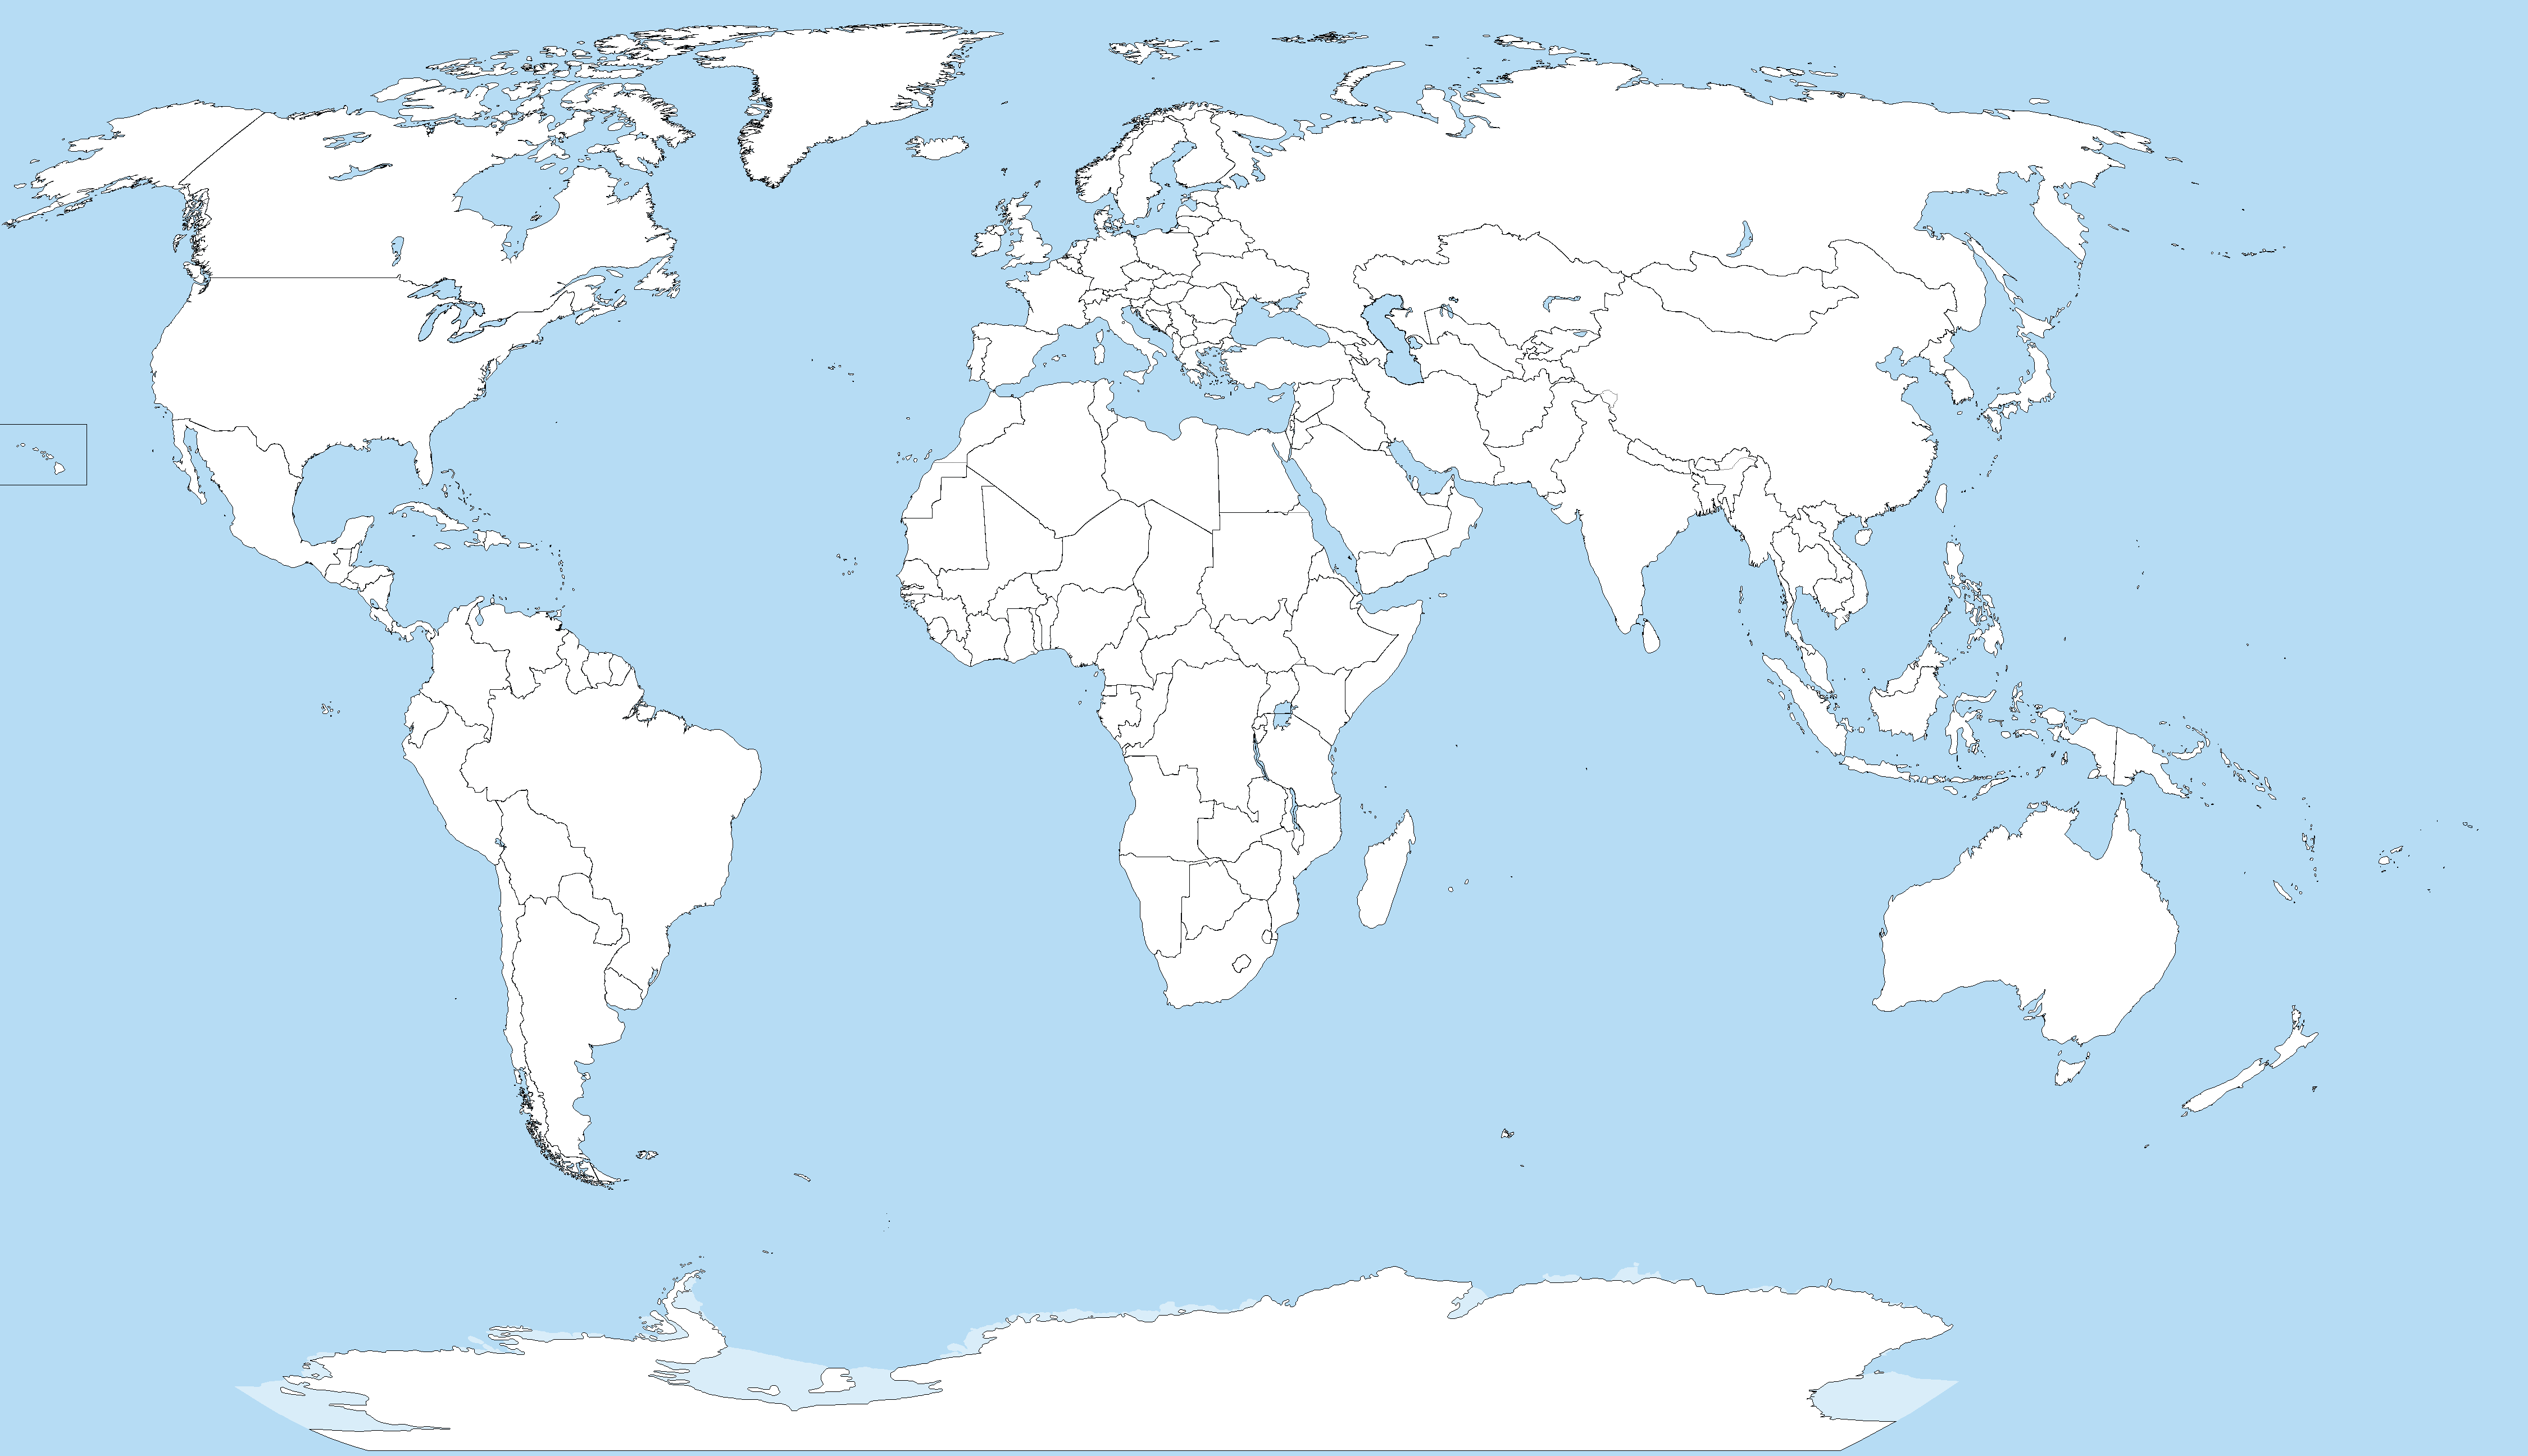
\includegraphics[width=0.7\textwidth]{worldmap.png}
	\end{figure}
	I had to perform numerous tasks to alter the map appropriately to have everything with the correct proportions that included:
	\begin{itemize}
		\item Resizing Europe, Asia, \& Africa
		\item Erasing Numerous Islands
		\item resizing greenland
		\item redrawing most borders to make the appropriate 42 regions,
		\item recoloring the territories to make the continents prominent
	\end{itemize}
	Once I had completed this, I needed to then make it so it was possible to click the region and for the game to know what it was. I achieved this by creating Polygon Colliders for every single Territory. This required me to manually make them follow the borders as closely as possible which was very time consuming. I utilized the special quality of islands and I was a bit more relaxed with how they are laid out and they are just irregular polygons (Unless they have a Land border where that is following the border as closely as possible) Here are some of them highlighted below:
	\begin{figure}[h!]
		\centering
		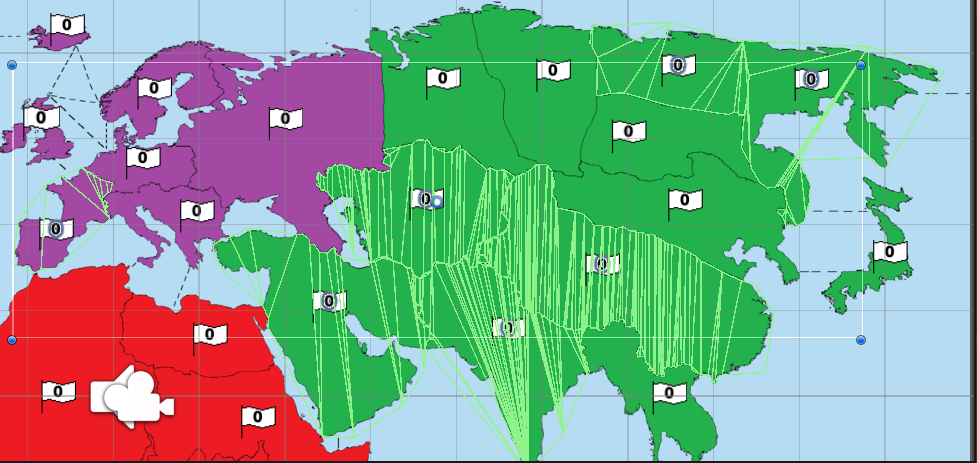
\includegraphics[width=0.7\textwidth]{colliders.png}
	\end{figure}
	Then In order to get the Region The Mouse was over, I used RayCastHit2D to see if I hit anything then performed some checks to see if the collision was valid.\\ I later realized that it was somewhat difficult to figure out what Territory I had clicked on So I made a Method for the Province Class that each province held that created a line renderer that followed the borders set out by the already existing polygon colliders as a nice visual reference for the player. Here is a demonstration where I click on afghanistan:
	\begin{figure}[h!]
		\centering
		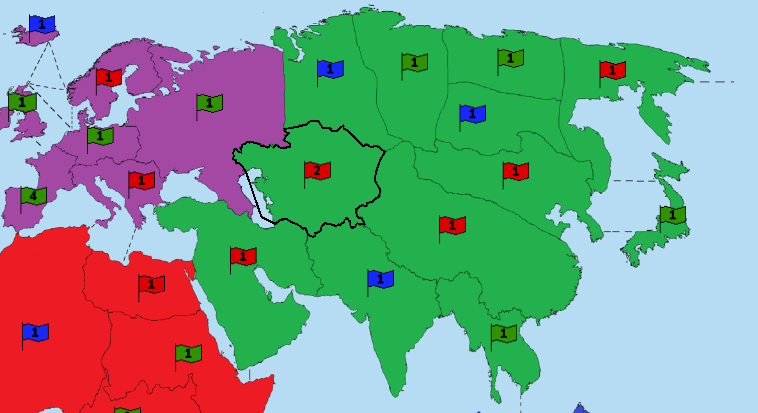
\includegraphics[width=0.7\textwidth]{linerendererdemo.png}
	\end{figure}
	This screenshot leads to the next section
	\newpage
	\subsection{Making the flags}
		\begin{figure}[h!]
			\centering
			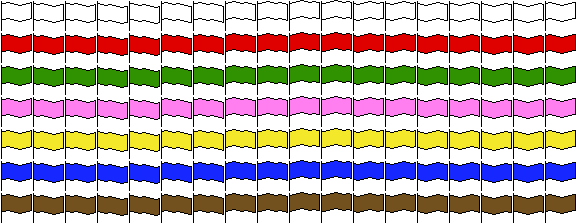
\includegraphics[width=0.7\textwidth]{flagsheet.png}
		\end{figure}
		In order to make the flags I used GIMP to make a 32x32 flag, I wanted to make it animated so I created a Flag waving animation to the best of my ability. So Then I duplicated it seven times and added unique colors. I then made seven Unity animations using this spritesheet I created. I was now faced with a new Issue which leads me to the next point.
	\subsection{Changing the flags color}
		\textit{Abandon all hope, ye who enter here}\\
		\begin{figure}[h!]
			\centering
			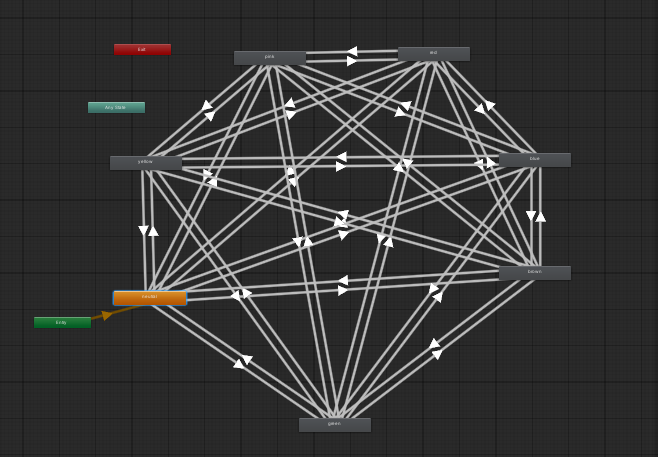
\includegraphics[width=0.5\textwidth]{animationTree.png}
		\end{figure}
		In order to make it transition between the flags when changing teams I had to make an animation tree, sadly AnyState would not allow the transitions to match the behavior I wanted(They kept transitioning mid animation) I hard coded all 36 conversions. The way I did this was I made an AnimationController with one varible: Team, this was kept as an integer and each value corresponds to a different flag and then if the value changes, it goes to the appropriate flag and so on.
	\subsection{Making the Dice}
		\begin{figure}[h!]
			\centering
			
\includegraphics[width=0.75\textwidth]{dice.png}
		\end{figure}
		I made a 32x32 dice in GIMP and then made all six faces and then an alternative color for the attack dice
	\newpage
	\section{Making the menus}
		\begin{figure}[h!]
			\centering
			\begin{minipage}[c]{0.5\textwidth}
				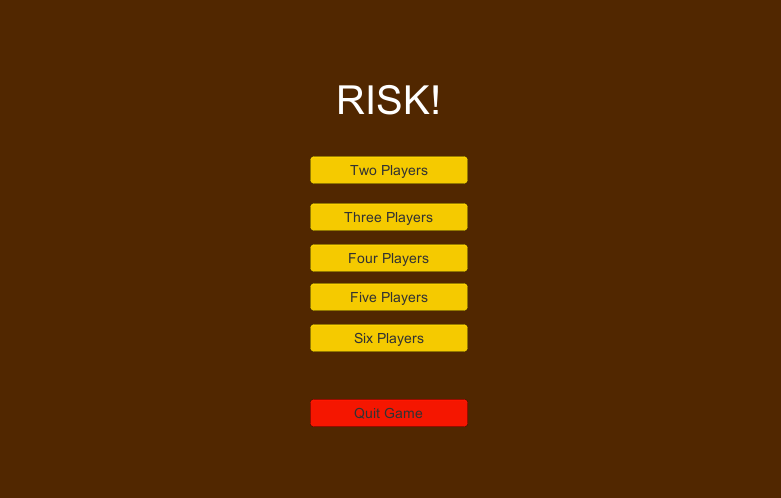
\includegraphics[width=0.9\textwidth]{mainMenu.png}
			\end{minipage}%
			\begin{minipage}[c]{0.5\textwidth}
				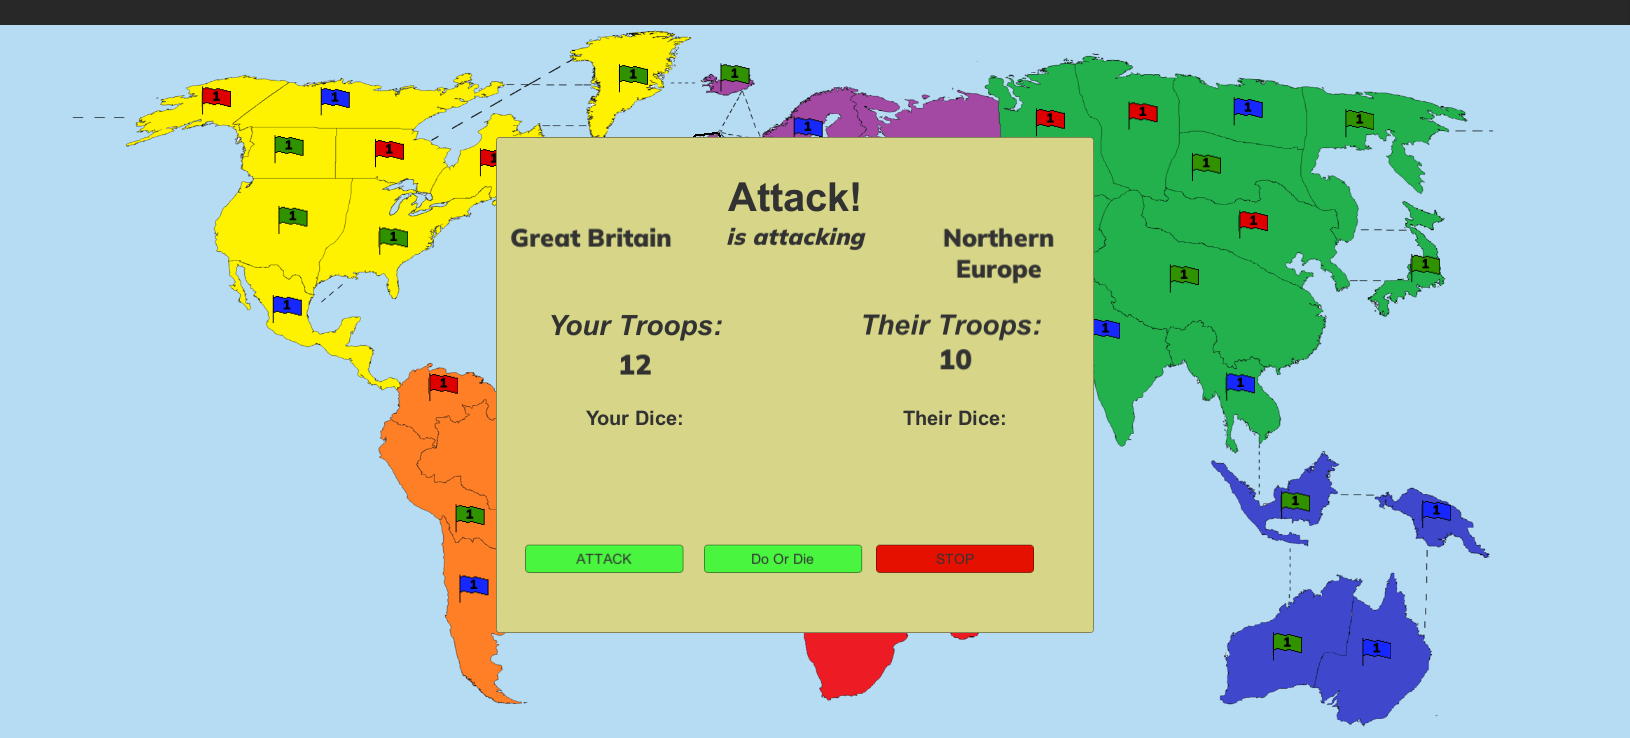
\includegraphics[width=0.9\textwidth]{prog2.png}
			\end{minipage}
			\begin{minipage}[c]{0.5\textwidth}
				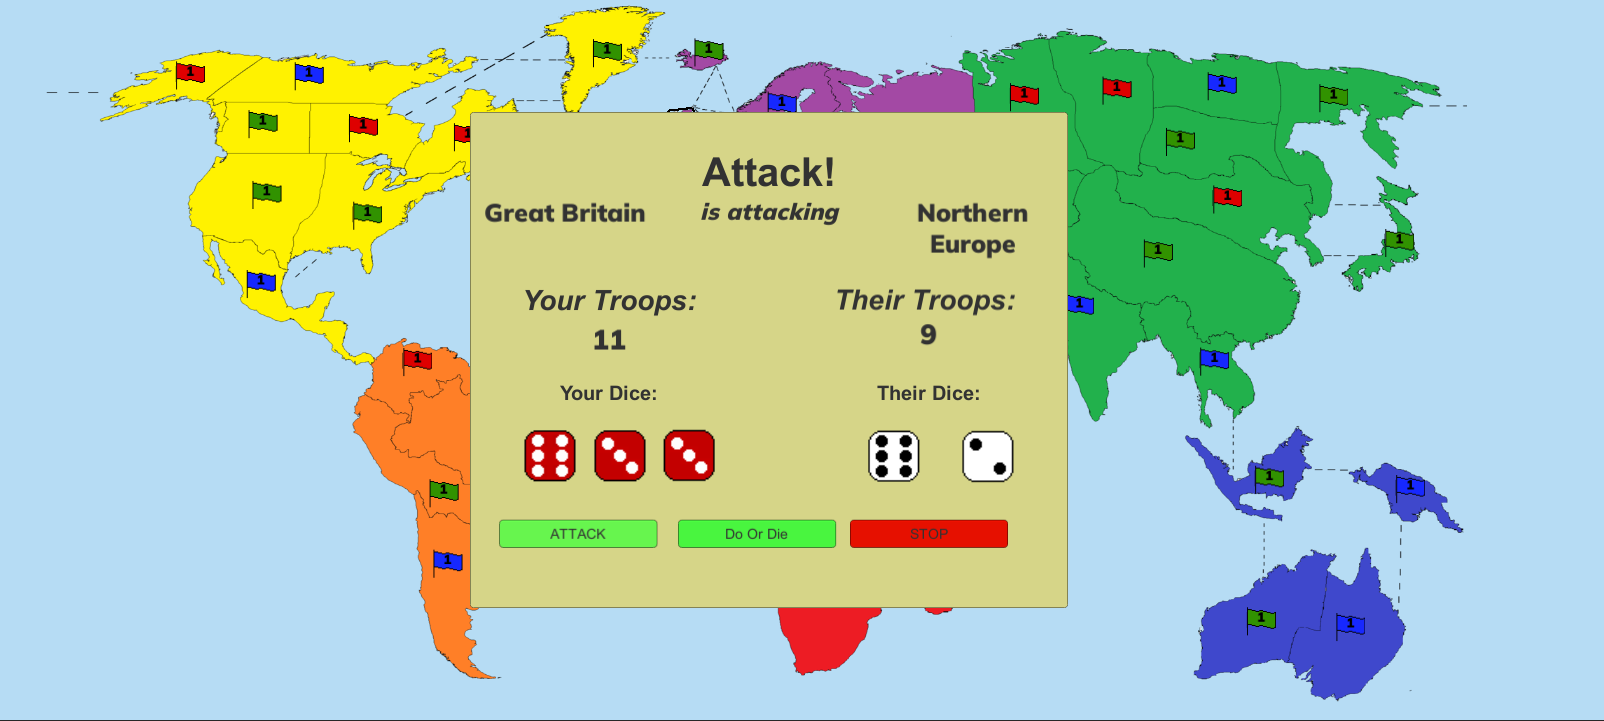
\includegraphics[width=0.9\textwidth]{prog3.png}
			\end{minipage}%
			\begin{minipage}[c]{0.5\textwidth}
				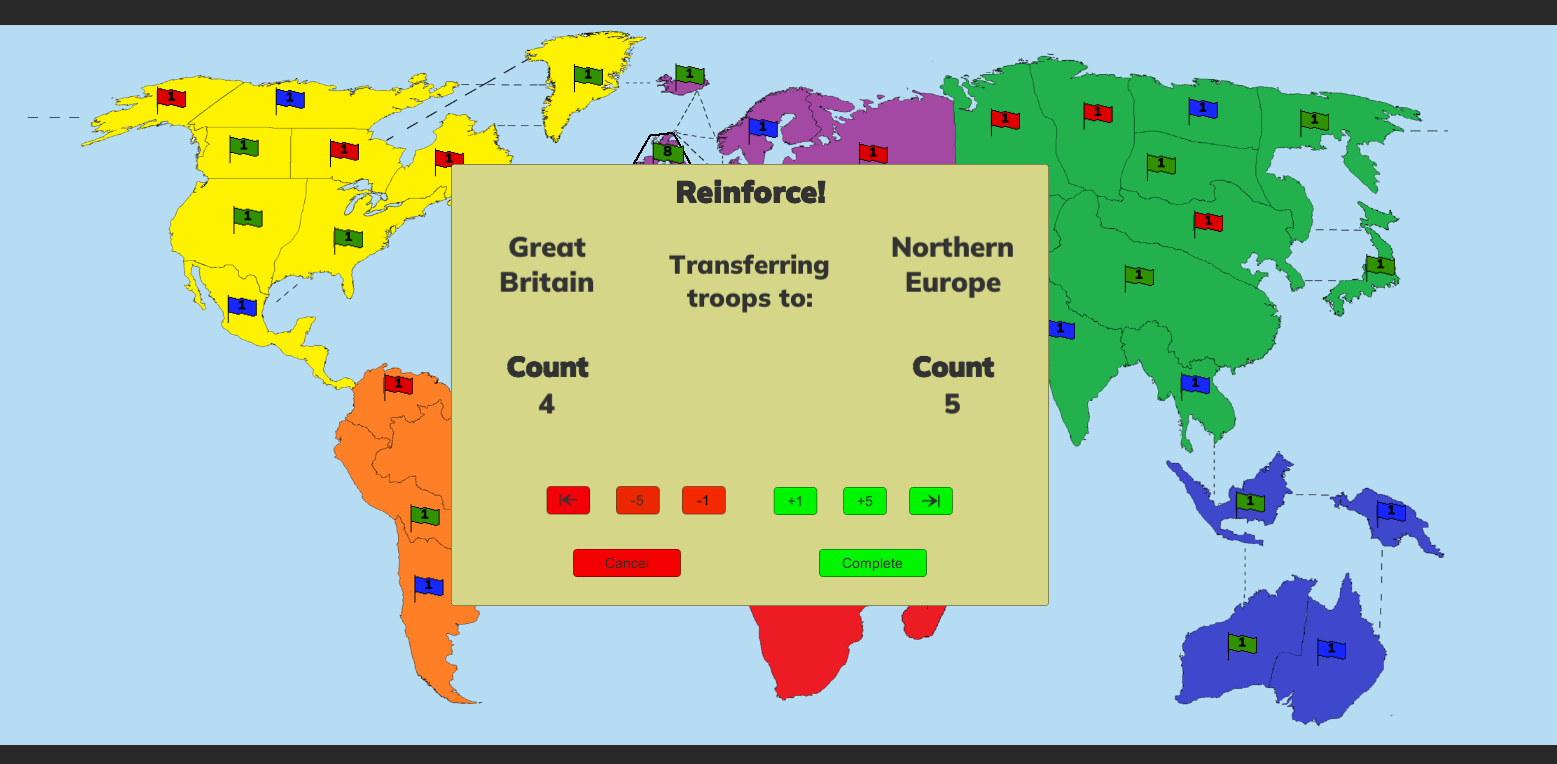
\includegraphics[width=0.9\textwidth]{prog4.png}
			\end{minipage}
		\end{figure}
		The Menus were very straight forward for the most part, as they were primarily consisted of buttons, apart from teh dice. The Dice were made by making panels with dice faces as images. Each Dice was attached to a Dice Class that was made and when you Invoked Dice.Roll() it automatically updated the faces of the dice.
	\section{The Game Itself}
	Now once all the UI has been shown. I will now go over the turn logic
	\subsection{Setup}
		As Risk has two ways of setting up (Either the players pick territories one by one, or they are distributed fairly at random), I Opted for the distribution at random option as I figured that it would be easier to implement.
		I do however, still have to allow them to populate these regions one by one at the end of the setup phase.
	\subsection{Your Turn}
		\subsubsection{Replenish}
			In order to replenish a calculation must be performed to get the number of troops you can distribute. This is done in the same way as the physical variant of risk. That being that the amount of territories you possess are divide by three and rounded down and this value or three whichever is greater, is then added to contenential bonuses (These are done by having each continent in a list and I check to see if that list is a subset of all the territories owned by a given player, if it is then the award is granted). You then have to distribute the troops you were awarded here before the beginning of the next phase.
		\subsection{Attack}
			The attack form stage is fairly straightforward, you click on a territory if it belongs to you it becomes marked. Then if you selected a territory that is not your own afterwards, an adjacency check is performed and if it is not met then you cannot attack, otherwise the attack interface shows up. If you happen to click on a territory of your own after already selecting a territory of your own, the previously selected territory is replaced with this. If you win the battle a reinforcement interface shows up which allows you to move troops to your newly conquered territory without ending your turn.
		\subsection{Reinforce}
			this is the final phase of the Turn. This allows you to move units from one territory to another so long as some connected path exists, and you own both territories. A path is calculated using a simple Depth First Search that I made and then if a path exists then the reinforcement interface shows up, and when this reinforcement ends, your turn concludes. A check is performed to see if anyone owns all 42 territories and if they do you are booted to the menu and the game concludes.
			
	\subsection{What is not here/issues}
		I struggled to calculate an appropriate timeframe for the game and ultimately the UI Design took far longer than I anticipated, so I ended up making this a local hotseat game as I did not have enough time to implement AI. All else that Is missing is a territory card system.\\
		Additionally, the game appears somewhat squashed on some monitors as I forgot to account for a 16:9 Aspect Ratio and I ended up forcing a 23:9 ratio to ensure that the entire map was visible.
		
	\section{Reflection}
		Overall this was a very educational experience where I learned a lot about games and project management. I am tempted to keep working on the game and try implement an AI as I reckon it would be pretty fun to do.
		
	\section{Code}
	\subsection{Game Manager Script}
	\cscode{GameManagerScript.cs}
	\subsection{Dice Roller}
	\cscode{DiceRoller.cs}
	\subsection{Province}
	\cscode{Province.cs}
			
	%Sets to Harvard Style and links the references file
	\bibliographystyle{agsm}
	\bibliography{references}
\end{document}